\documentclass[mcp]{article}
%\documentclass[11pt, twocolumn]{article}

\usepackage[colorinlistoftodos]{todonotes}
\usepackage{graphicx}
\graphicspath{ {./images/} }

\usepackage{fullpage}
\usepackage{amsfonts,amsthm}
\usepackage{amsmath}
\numberwithin{figure}{section} % numbering in each subsection
\numberwithin{table}{section}
\usepackage{setspace}
\usepackage{url}
\usepackage{lscape} %% rotating table
\usepackage{rotating}
\usepackage{hyperref}
\usepackage{xcolor} %\[table,dvipsnames]
%\usepackage{makecell}
%\usepackage{array}

% remove number of section in the title
\makeatletter
\def\@seccntformat#1{%
  \expandafter\ifx\csname c@#1\endcsname\c@section\else
  \csname the#1\endcsname\quad
  \fi}
\makeatother

\usepackage{caption}

%% to remove zero preceding section number.
\renewcommand\thesection{\arabic{section}}
\renewcommand\thesubsection{\thesection.\arabic{subsection}}

\usepackage{tabulary,multirow,multicol,rotating}
\usepackage[backend=biber]{biblatex}
\addbibresource{bibliography.bib}

\definecolor{Red}{rgb}{0.60,0.00,0.00}
\definecolor{Blue}{rgb}{0.00,0.00,0.75}
\definecolor{LightYellow}{rgb}{1.00,0.97,0.68}
\definecolor{Green}{rgb}{0.30, 0.60, 0.30}
\definecolor{MyLightMagenta}{cmyk}{0.1,0.8,0,0.1} 
\definecolor{cornflowerblue}{rgb}{0.39, 0.58, 0.92}
\definecolor{darkorange}{rgb}{0.8, 0.4, 0}
\definecolor{LightPurple}{rgb}{1, 0.51, 0.98}
\definecolor{DarkPurple}{rgb}{0.54, 0.27, 0.53}
\definecolor{Purple1}{rgb}{0.83, 0.29, 0.95}
\definecolor{Purple2}{rgb}{0.97, 0.12, 0.59}
\definecolor{change}{rgb}{0.39, 0.58, 0.92}

\definecolor{function}{RGB}{0, 112, 192}
\definecolor{group}{rgb}{0.39, 0.58, 0.92}
\definecolor{ratio}{rgb}{1, 0.6, 0.16}
\definecolor{feature}{rgb}{0.83, 0.32, 0.48}
\definecolor{subject}{rgb}{0.6, 0.3, 0.09}
\definecolor{run}{rgb}{0, 0.68, 0.17}

\usepackage{array}
\newcolumntype{C}[1]{>{\centering\let\newline\\\arraybackslash\hspace{0pt}}m{#1}}
\setlength{\tabcolsep}{2pt}

%% for comments
\newcommand{\ignore}[1]{}
\def\todo#1{{\color{red}[#1]}}
\def\change#1{{\color{cornflowerblue}#1}}
\newenvironment{todolong}{\color{red}[TODO:}{]}
\def\note#1{{\color{OliveGreen}[NOTE: #1]}}
\def\added#1{{\color{blue}[ADDED: #1]}}
\def\devon#1{{\color{green}[4Devon: #1]}}

\def\eqref#1{Eq.~(\ref{eq:#1})}
\def\figshortref#1{{\bf Fig.~\ref{fig:#1}}}
\def\figref#1{{\bf Figure~\ref{fig:#1}}}
\def\secref#1{{\bf Section~\ref{sec:#1}}}
\def\tabref#1{{\bf Table~\ref{tab:#1}}}

\usepackage{xr}
\externaldocument[supp-]{ptm_sm}
%\def\sfigref#1{{\bf Supplementary Fig.~\ref{fig:#1}}}
%\def\snoteref#1{{\bf Supplementary Note~\ref{sec:#1}}}
%\def\snoteshortref#1{{\bf Suppl. Note~\ref{sec:#1}}}
%\def\stabref#1{{\bf Supplementary Table~\ref{tab:#1}}}

%%% should be change =2
\linespread{1}

%\date{\vspace{-5ex}} % to remove date in the title

\renewcommand{\deg}{\ensuremath{^{\circ}}\xspace}


%%%%%%%%%%%%%%%%%%%%%%%%%%%%%%%%%%%%%%%%%%%%%%%%%%%%%%%%%%%%%%%%%%%%%%%
%%%%%%%%%%%%%%%%%%%%%%%%%%%%%%%%%%%%%%%%%%%%%%%%%%%%%%%%%%%%%%%%%%%%%%%
%%%%%%%%%%%%%%%%%%%%%%%%%%%%%%%%%%%%%%%%%%%%%%%%%%%%%%%%%%%%%%%%%%%%%%%

\title{Statistical methods for relative quantification of post-translational modifications in global proteomics experiments}

%\author{
%  LastName1, FirstName1\\
%  \texttt{first1.last1@xxxxx.com}
%  \and
%  LastName2, FirstName2\\
%  \texttt{first2.last2@xxxxx.com}
%}
\date{}
\begin{document}

\maketitle
\todo{Add Author list}
%\noindent\author{Tsung-Heng Tsai$^{1}$, Olga Vitek$^{1,\ast}$}
%
%\vspace{0.2in}
%\noindent $^1$   Khoury College of Computer Sciences, Northeastern University, Boston, MA, USA\\
%\noindent $\ast$   Corresponding author \\

\devon{maybe good to have supplementary.txt in the same folder, to link figure, table number between main and supplementary.}

%%%%%%%%%%%%%%%%%%%%%%%%%%%%%%%%%%%%%%%%%%%%%%%%%%%%%%%%%%%%%%%%%%%%%%%
%%%%%%%%%%%%%%%%%%%%%%%%%%%%%%%%%%%%%%%%%%%%%%%%%%%%%%%%%%%%%%%%%%%%%%%
\section{Abstract}

The scientific community widely utilizes mass spectrometry (MS)-based proteomics to quantify the abundance of proteins and their post-translational modifications (PTMs). Experiments targeting PTMs face several specific challenges. These include the low abundance of modified proteo-forms, few representative peptides that span modification sites, and convolution with abundance changes in the overall protein expression. Due to these challenges, a robust approach to estimate relative systematic changes in PTMs should combine information pertaining to PTM sites over several peptides, replicates in multiple conditions, and consider sources of confounding and variation present in the experiment. We propose a general statistical model and workflow that is both reproducible and comprehensive. The model measures PTM and protein abundance by summarizing intensities through Tukey’s median polish method. Then a model based on the family of linear mixed-effects models is fit. This model is automatically adjusted to the specific experimental design. Finally, the PTM abundances are adjusted to remove variance from changes in the overall protein. We implement this model in the free and open-source R package MSstatsPTM.


%%%%%%%%%%%%%%%%%%%%%%%%%%%%%%%%%%%%%%%%%%%%%%%%%%%%%%%%%%%%%%%%%%%%%%%
%%%%%%%%%%%%%%%%%%%%%%%%%%%%%%%%%%%%%%%%%%%%%%%%%%%%%%%%%%%%%%%%%%%%%%%
\section{Introduction}

The signaling mechanisms that allow cells to mount a dynamic and fast response to a multitude of events are primarily facilitated by the modification of proteins at specific residues, acting as molecular on/off switches.\cite{Deribe} \cite{Cohen}  Mass spectrometry-based label-free proteomics is broadly established as the tool-of-choice for unbiased and large-scale identification and quantification of proteins and their post-translational modifications (PTMs) using liquid chromatography coupled with mass spectrometry (LC-MS)\cite{Kall:2011ub} \cite{Roepstorff}. Studies targeting the post-translationally modified proteome focus either on the accurate localization of modification sites on proteins, relative or absolute quantification of a modification site’s occupancy repertoire, or relative changes in occupancy across experimental conditions.\cite{Mann} Regardless of the question at hand, interrogating the modified proteome is challenging due to a number of reasons. First, the relatively lower abundance of modified proteo-forms dictates that a global interrogation can only be achieved through large-scale enrichment protocols with modification-specific antibodies or beads. Variability in the enrichment efficiency inevitably affects the reproducibility of the number of spectral features (e.g., peptide precursor ions or their fragments) and their intensities, which imposes challenges in both quantification and statistical modeling. Second, contrary to the often large number of identified peptides that can be used as features to model protein abundance changes, there are relatively few representative peptides that span a modification sites, which often results in sparse, and sometimes, inherently convoluted models (i.e., single versus multiple modified sites on a single peptide). Third, unless early signaling events are interrogated, the interpretation of the relative changes in modification occupancy are inherently convoluted with changes in the overall protein expression, making the interpretation of the results not straightforward. \cite{Olsen:2013} Therefore, a robust approach to estimate systematic relative changes in post-translational modifications, at scale, should not only combine the quantitative information pertaining to a PTM site over peptides and replicates in multiple conditions, but take into account various sources of variations and confounding factors present in the experiments.

Despite the important implications of PTMs in biological functions, there is a lack of general framework to summarize the available quantitative information from LC-MS data, to perform statistical inference, and to draw conclusions to characterize the quantitative properties of PTM in a statistically rigorous manner. Many investigations performed differential expression analysis of PTMs using two-sample t-test or its extensions. \todo{Add Ref about current PTM approaches} The approach takes as input intensities of individual features from modified peptides, or intensity ratios of modified and unmodified peptide features, and compares the mean abundance of a PTM site from one condition to another. Modifications of the t-test such as moderated t-test with limma were also proposed.\cite{Zhu} While simple, the approach does not fully account for the sources of variations, and it is not directly applicable to experiments with complex designs, e.g., comparisons of multiple conditions, acquisition in multiple batches, etc. Isobar-PTM was developed for experiments with MS/MS quantitative strategies that employ isobaric labels such as tandem mass tags (TMT) and isobaric tag for relative and absolute quantification (iTRAQ).\cite{Breitwieser:2013} Isobar-PTM expresses MS measurements with a linear model and performs adjustment with respect to protein abundance using the difference between log-ratio of modified peptides in two channels and log-ratio of protein level. The modeling framework, however, is not applicable for either label-free workflows or experiments with complex designs.

We propose a general statistical approach, which explicitly characterizes the variations and confounding factors present in bottom-up PTM experiments. The proposed approach is aimed at the detection of quantitative changes in PTMs between conditions utilizing procedures developed for summarization of LC-MS data, quantitative characterization of site-specific PTMs, and adjustment with respect to protein abundance. Quantitative analyses of PTMs often involve comparisons between multiple inter-related conditions of the same biological system. The general statistical framework underlying the proposed approach allows for analyzing experiments with complex designs, including those with multiple conditions, multiple batches, and measured at different points in time. 

The proposed approach was evaluated using datasets from computer simulations, benchmark controlled mixtures, and biological investigations. The approach was then compared against the commonly applied t-test. The results demonstrate that by appropriately leveraging the information from the entire dataset the proposed approach improves the reproducibility and accuracy of the estimates of PTM fold changes, results in a better calibrated type I error rate, and improves the statistical power of detecting changes in PTMs. The proposed approach is implemented as an open source R package MSstatsPTM, which employs similar input format as in MSstats and MSstatsTMT \cite{Choi:2014} \cite{Huang:2020}.

%%%%%%%%%%%%%%%%%%%%%%%%%%%%%%%%%%%%%%%%%%%%%%%%%%%%%%%%%%%%%%%%%%%%%%%
\section{Proposed Approach}

\todo{Not sure what to do with this part and figure. How would this look in a paper?}
Figure \ref{fig:data-structure} schematically illustrates a simplified version of the data structure resulting from a typical bottom-up experiment for quantitative analysis of PTMs, in which there are multiple layers of variation present. A PTM site is quantified with multiple spectral features, which vary in sequence (e.g., fully or partially cleaved peptides), ionization efficiency, charge states, etc. The number quantified features vary across replicate LC-MS/MS runs of the same sample, and across conditions. To perform adjustment with respect to protein abundance, features of unmodified peptides are used for the inference of underlying protein abundance. Typically, because of the enrichment step for PTMs, very few of those features are present in original LC-MS runs. For more accurate estimation of protein abundance, separate global proteomics data of unenriched samples are often acquired. As different levels of variability are present in the data, the log-intensities of the features for modified and unmodified peptides are modeled separately using two linear mixed models. 

%%%%%%%%%%%%%%%%%%%%%%%%%%%%%%%%%%%%%%%%%%%%%%%%%%%%%%%%%%%%%%%%%%%%%%%
\subsection*{Statistical modeling and parameter estimation}

The proposed approach takes as input a list of log-transformed intensities of spectral features, identified and quantified across LC-MS runs. The features, which are precursor ions of modified or unmodified peptides, are used to characterize the identified PTM sites and proteins. For each PTM site, the feature log-intensities of the modified peptides spanning the site are expressed using a linear mixed model in consideration of the effects of condition, run, feature and interaction between run and feature. The model parameters are estimated using the split-plot approach as in MSstats, where the feature log-intensities are first summarized into a single value per site per run in the subplot model, and the site-level summaries are then used for the inference of the PTM site abundance.\cite{Choi:2014} In the site-level summarization, Tukey's median polish (TMP), a simple and robust procedure is applied to iteratively fit a two-way additive model with the effects of run and feature, which in turn summarizes the log-intensities for each site.\cite{Tukey:1977} After summarization, the inference of the PTM site abundance in each condition is carried through fitting a model based on the family of linear mixed-effects models, taking into account the specific experimental design \ref{fig:data-structure}.\cite{Bolker2009} \cite{Faraway:2006} Statistical modeling and quantification for global proteomics data are performed by the same procedure as for PTM data.

%%%%%%%%%%%%%%%%%%%%%%%%%%%%%%%%%%%%%%%%%%%%%%%%%%%%%%%%%%%%%%%%%%%%%%%
\subsection*{Detection of changes in PTMs}

Detection of differentially modified PTM sites is performed through testing the null hypothesis of ‘no change’ against the alternative. The null hypothesis states that there is no difference in log-abundance of the PTM site between conditions, adjusted with respect to protein abundance \ref{fig:data-structure}. Specifically, the adjusted difference is given by the difference in log-abundance of the PTM site, subtracted by the difference in log-abundance of the underlying protein, which is equivalent to the log of the ratio of PTM abundance difference to protein abundance difference. The estimate of the adjusted difference and the standard error (SE) of the estimate are obtained by combining the difference estimates and the associated SEs from both counterparts. The standard error of the estimate $\mathrm{SE}(\hat{\Delta})$ is 

\[
\left[ \frac{2}{J} \left( \hat{\sigma}_{\gamma}^{2} + \hat{\sigma}_{\gamma^{\ast}}^{2} \right) \right]^{1/2}.
\]

The test statistic for the hypothesis testing is the ratio of the estimate of the adjusted difference to its SE. To determine the statistical significance of the difference in terms of p-value, the test statistic is compared against the t distribution with degrees of freedom approximated by the Satterthwaite method. \cite{satterthwaite:1946} Adjustment for multiple comparisons is performed using the Benjamini-Hochberg procedure to control the false discovery rate at a desired level, e.g., 0.05.\cite{Benjamini:1995} The details are provided in Supplementary Sec. S3.2 \devon{link to supplementary using sfigref}.

%%%%%%%%%%%%%%%%%%%%%%%%%%%%%%%%%%%%%%%%%%%%%%%%%%%%%%%%%%%%%%%%%%%%%%%
\subsection*{Analysis with multiple batches}

The proposed statistical framework allows to analyze data from experiments of complex designs such as factorial design. We discuss below a specific design commonly considered in PTM experiments, in which data are acquired in multiple batches, often as a result of multiple repeats for the antibody enrichment step. Typically, the number of spectral features and their intensities are different across batches, and the run-to-run variation sometimes varies across batches as well. The proposed approach summarizes log-intensities in each batch separately, and considers two ways to perform the statistical inference and testing. When variability in site-level summaries and in PTM changes is expected across batches, the proposed approach performs inference of the PTM site abundance and the adjusted difference for each batch separately. The evidence about differential PTM sites between conditions is averaged over batches. Alternatively, assuming identical variability in the site-level summaries and identical differences between conditions across batches (i.e., no interaction effect between condition and batch), the statistical inference and testing can be performed based on one single model with an additional fixed effect of batch. Details about these modeling considerations are discussed in Supplementary \todo{link to Sec. S3.4}.

%%%%%%%%%%%%%%%%%%%%%%%%%%%%%%%%%%%%%%%%%%%%%%%%%%%%%%%%%%%%%%%%%%%%%%%
\subsection*{Missing Value imputation}

MSstatsPTM gives the ability to impute missing feature intensities if desired. When values are imputed, it is assumed they are missing for reasons of low abundance. Missing features are imputed in each MS run using the Accelerated Time Failure model.\cite{Tukey:1977} In order to impute a feature's missing values, the feature must be present in at least one MS Run. If the feature is not present across all MS Runs, the value will be left missing. Missing value imputation is done before summarization with Tukey's Median Polish in order to correct for the impact of outliers. Missing value imputation is done separately for both the PTM and global protein datasets.

%%%%%%%%%%%%%%%%%%%%%%%%%%%%%%%%%%%%%%%%%%%%%%%%%%%%%%%%%%%%%%%%%%%%%%%
\subsection*{Extension to TMT experiments}

The statistical modeling approaches discussed above can also be extended to Tandem Mass Tag (TMT) labeling methods. TMT experiments introduce an additional source of variation in the form of different mixtures. To account for the mixture variable, first feature intensities are summarized as described previously, then a new linear mixed effects model with an added term for the mixture is included. This workflow and model follow the methods used for MSstatsTMT. \cite{Huang:2020} These methods are repeated to quantify and model global protein abundance. Once both PTM and global protein are modeled, the PTM model is adjusted for changes in global protein abundance using the same methods are before.

\todo{add figref for TMT model}
\todo{add figref for TMT experiment table}

%%%%%%%%%%%%%%%%%%%%%%%%%%%%%%%%%%%%%%%%%%%%%%%%%%%%%%%%%%%%%%%%%%%%%%%
%%%%%%%%%%%%%%%%%%%%%%%%%%%%%%%%%%%%%%%%%%%%%%%%%%%%%%%%%%%%%%%%%%%%%%%
\section{Results}

\subsection*{Computer simulations}

The proposed statistical approach methods were evaluated using computer simulation. Specifically, their properties under adjustment with respect to protein abundance and batch effects were evaluated.

\paragraph*{Computer simulation: protein-level adjustment.} 

Differential intensity levels of modified peptides may be due to changes in modification, change in protein abundance, or both. The proposed approach adjusts the abundance with respect to unmodified peptides by combining the inference of modified and unmodified peptide abundances. Alternatively, two-sample t-test that takes as input the ratio between modified and unmodified peptide intensities (difference on log scale) is commonly applied for the same purpose. In real experiments, multiple inter-related conditions are often compared together. Whereas t-test uses measurements from the two conditions being compared, the proposed approach leverages measurements in all conditions for the inference of underlying abundance. We evaluated the impact with such adjustment by computer simulation, considering the following factors: with/without protein-level changes, effect size, number of replicates and number of conditions. Details of the simulation can be found in Supplementary \todo{link to Sec. S4.1}. 

In this simulation, when there was no change in protein abundance, all the considered approaches well calibrated the Type I error rate \todo{figref Fig. 4a}. However, when the modification changes were entirely due to the changes in protein abundance across conditions, analysis without accounting for the protein-level changes resulted in off-target, high false positive rates \todo{figref (Fig. 4b)}. As shown in \todo{figref Fig. 4c-e}, in detection of systematic changes in PTM abundance, the proposed approach improved statistical power with small sample sizes in almost all the considered scenarios. The advantage by using the proposed approach over t-test became more profound in the presence of missing data \todo{figref (Fig. 4d-e)}. In cases with small sample sizes (e.g., 2 replicates) as shown in \todo{figref Fig. 4d}, performance by t-test decreased dramatically with one missing value, and increasing the log-fold change to 2 did not effectively reduce the negative impact. Two-sample t-test only used data within the groups of interest while ignoring the rest of the data. Consequently, it gave similar performance across cases with different number of conditions. In contrast, the proposed approach leveraged all available information, which resulted in improved power with increased number of conditions (see for example, the improved performance in \todo{figref Fig. 4e} [with 4 conditions] over \todo{figref Fig. 4d} [with 2 conditions]). Further results are provided in Supplementary \todo{link to Sec. S4.1}. 

\paragraph*{Computer simulation: batch effects.} 

PTM experiments often create batches during data acquisition. The proposed approach can be naturally extended to handle such scenarios by modeling various forms of batch effects, as a t-test is not directly applicable to a problem with batches of data. Two commonly used ad-hoc approaches are a) t-test (no batch): ignoring batch effects when applying t-test, and b) t-test (most significant batch): applying t-test in each batch and drawing conclusions based on the most significant batch.\todo{Find source for batch analysis} Although simple, these ad-hoc methods lack statistical justification. We characterized their statistical properties under various forms of batch effects in Supplementary \todo{link to Sec. S4.2}. Two batches of data were generated, where various forms of batch effects were simulated, including difference in signal intensities across batches, difference in variability across batches, and interaction between batch and condition (i.e., change between conditions affected by batch). 

The major results are summarized in \todo{figref Fig. 5} with additional details provided in Supplementary \todo{link to Sec. S4.2}. In terms of estimation of fold change, the most statistically significant batch with t-test was highly variable and frequently biased (Fig. 5a). In the detection of systematic changes in PTM abundance, it also frequently resulted in higher false positive rates than the expected value (Fig. 5b). As shown Fig. 5c, the proposed approach improved power with small sample sizes in almost all the scenarios, under various forms of batch effects including difference in intensity level and difference in variability. Using t-test while ignoring batch effect gave similar performance in special cases with no difference in intensity level between batches (Supplementary Fig. \todo{find and link this section SXX}), but its performance dramatically decreased in general cases (Supplementary \todo{link to Figs. S8-S9}). The negative impact was only partially reduced by increasing the sample size to 5. The proposed approach gave consistently improved performance compared with other methods by properly characterizing batch effects and leveraging all available information.

%%%%%%%%%%%%%%%%%%%%%%%%%%%%%%%%%%%%%%%%%%%%%%%%%%%%%%%%%%%%%%%%%%%%%%%
\subsection*{Spike-in experiment}
\todo{Need to write results of this experiment}

We evaluated our approach using a custom designed spike-in benchmark experiment where 50 heavy-labeled KGG motif peptides from 20 human proteins were used as spike-in peptides. Quantitative changes in protein and site abundance changes of these 20 proteins were the target of the benchmark. Unmodified peptides from Human Lysate were used as the estimate of global protein abundance changes. All comparisons with respect to human lysate serve as a null model, there was no change in global protein nor PTM abundance between conditions. Additionally, E coli Lysate was used to normalize total protein levels prior to enrichment or global protein profiling. Four mixes of spike in peptides and Human Lysate were created to create conditions with known fold change. \todo{Add figure of mixtures} Two sets of data were acquired for each mixture: modifed peptide data, including the spike in KGG enriched peptides, and unmodified peptides from Human Lysate. These datasets were used as the PTM and global protein data.

\todo{figref volcano plot of spike in peptides}

In *FigXX* we can clearly see the red labeled spike-in peptides do not follow the expected fold change before adjusting for changes in global protein level. After adjustment the estimated fold change is much close to expectation. Additionally, background peptides that should not show a significant change, colored grey, show many false positives before adjustment is made. Again after adjustment the results improve, and the number of false positives decrease significantly. In this experiment adjusting to remove confounding with changes in global protein abundance leads to a more accurate conclusion about the effect of modified peptides between conditions.

%%%%%%%%%%%%%%%%%%%%%%%%%%%%%%%%%%%%%%%%%%%%%%%%%%%%%%%%%%%%%%%%%%%%%%%
\subsection*{Dilution experiment [What was this experiment?]}

We evaluated our approach using a custom designed dilution benchmark experiment where two sets of liver samples from five Atg16L1 deficient mice (one with KGG enrichment followed by trypsin digestion, one with trypsin digestion alone) were prepared. Following a randomized order, each sample was injected at three different concentrations 4ul, 2ul, and 1ul. The experiment resulted in 15 KGG and 15 global profiling runs. To correct for run-to-run variation, the AQUA peptide mixture was spiked into each sample. There are 4696 ubiquitinated proteins identified in this dataset. Among these, 3173 have corresponding measurements from global data.
To simulate the effects of changes in protein abundance, we created three groups of data by matching one concentration for the KGG data with one for the global data: K1P1, K2P2, and K4P4. Systematic changes in the abundance of ubiquitinated sites between the groups are present in the KGG data. These changes are considered as artifacts driven by the changes in the abundance of their corresponding proteins. Using the comparison of K2P2 vs. K1P1 as example, there are 19355 possible comparisons with KGG data, and 3860 changes are detected. Out of the 19355 sites, 15036 have corresponding measurements from global data and are eligible for protein-level correction. The correction significantly reduced the number of false positives to 79. Similar observations were made in the other two comparisons K4P4 vs. K2P2 and K4P4 vs. K1P1, as shown in Table XX. \todo{Create or find this table}

%%%%%%%%%%%%%%%%%%%%%%%%%%%%%%%%%%%%%%%%%%%%%%%%%%%%%%%%%%%%%%%%%%%%%%%
\subsection*{Re-analysis of published dataset: TMT experiment}

To evaluate our approach on TMT experiments we reanalyzed an experiment targeting primary murine macrophages infected with Shigella flexneri (S.flexneri). \cite{Maculins} Tandem mass tagging was used to quantify changes in total proteins, phosphorylation, and ubiquitination in Wild type (WT) controls and ATG16L1-deficient (cKO) bone marrow macrophages (BMDMs) either infected or uninfected with Shigella flexneri. 11-plex isobaric multiplex was used with two separate mixtures. Cell lysates were prepared over three different time periods, either uninfected, infected at early (45-60 min) or infected at late (3-3.5 hour) time points. There were 103,700 peptides mapping to 9,430 proteins in the global profiling run. Additionally, there were 25,600 unique phosphorylation sites and 12,400 KGG ubiquitination sites. About ~90\% of the identified modified peptides derived from proteins that were also quantified in the global profiling run.

The major results are summarized below.

%%%%%%%%%%%%%%%%%%%%%%%%%%%%%%%%%%%%%%%%%%%%%%%%%%%%%%%%%%%%%%%%%%%%%%%
%%%%%%%%%%%%%%%%%%%%%%%%%%%%%%%%%%%%%%%%%%%%%%%%%%%%%%%%%%%%%%%%%%%%%%%
\section{Conclusion and discussion}

We proposed a general statistical modeling framework for PTM characterization. The framework is designed for bottom-up MS workflows, which are characterized with variations from multiple convoluted sources, frequent missing data, and associated uncertainty in the conclusions. The framework is general and is applicable to a variety of experimental designs. It outperforms the ad-hoc methods underlying the t-test, and yields accurate results in the broad type of experimental circumstances, including the presence of missing values, changes in protein abundance, batch effects, and different acquisition methods. The framework allows us to plan for subsequent experiments, and choose the appropriate number of replicates in consideration of adjustment with respect to protein abundance. 

Our results show that when measurements from multiple related conditions are available, the proposed approach for joint modeling and summarization of all the LC-MS/MS runs leads to more sensitive PTM significance analysis and more accurate and precise quantification than when separately analyzing conditions of runs. The gain is due to a more efficient use of the data, and to a more accurate understanding of the systematic and random variations. The proposed framework can be extended beyond the experimental designs with multiple batches and conditions discussed above. For example, it can represent experimental designs with even more complex structures, such as time series or factorial investigations. 

A potential limitation of the proposed framework is the assumption that all the peptides are correctly mapped to the underlying proteins and PTM sites, and the features are informative of the abundances of underlying protein and PTM. Also, characterizing PTMs with current data-dependent acquisition workflows is prone to being under sampled, leading to a sparse dataset with a large number of missing values for the analysis. Statistical methods accounting for effects due to experimental units and missing values introduced in this manuscript help interpret the data in a more objective manner. The latest development of targeted acquisition and data-independent acquisition methods are expected to further alleviate these issues. 

Overall, the proposed approach balances accuracy and practicality, and enables the analysis of complex experiments in high throughput. Future work is to carry out the inference and testing for not only the relative change of PTM abundance, but also the fraction of the protein that is modified at the particular site (site occupancy, or stoichiometry). We are also interested in characterizing the interplay of PTMs at multiple sites. The proposed statistical methods are implemented as an R package MSstatsPTM available on Bioconductor and Github.


%%%%%%%%%%%%%%%%%%%%%%%%%%%%%%%%%%%%%%%%%%%%%%%%%%%%%%%%%%%%%%%%%%%%%%%
%%%%%%%%%%%%%%%%%%%%%%%%%%%%%%%%%%%%%%%%%%%%%%%%%%%%%%%%%%%%%%%%%%%%%%%

\section{Figure}

\begin{figure}[ht]
\centering
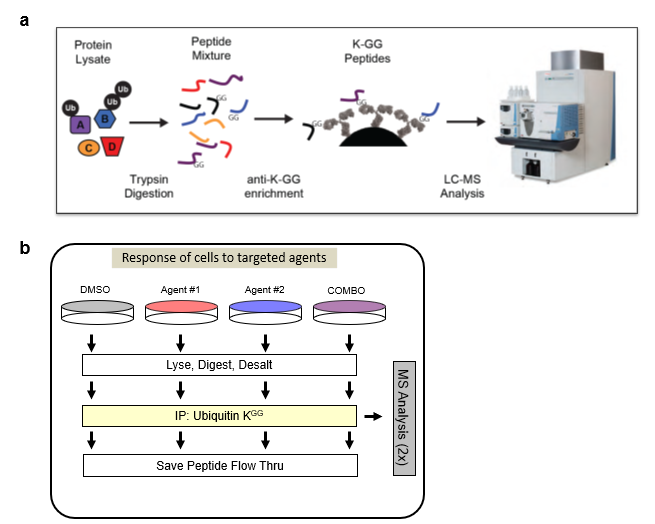
\includegraphics[scale=.8]{images/fig1.png}
\caption{}
\label{fig:workflow}
\end{figure}

\begin{figure}[ht]
\centering
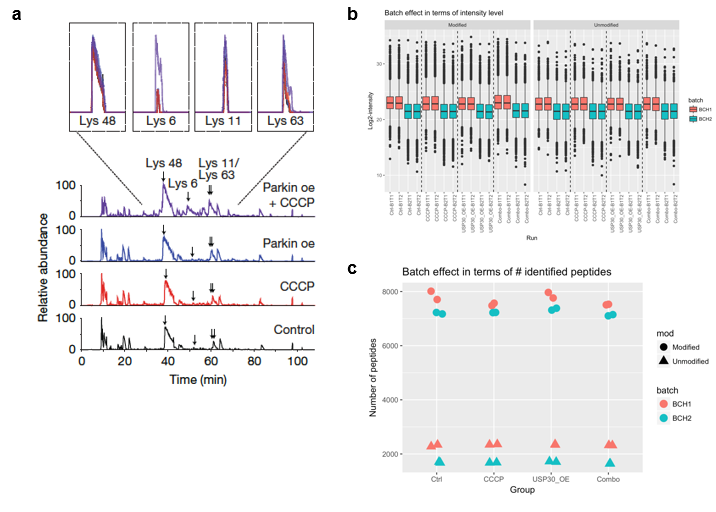
\includegraphics[scale=.8]{images/fig2.png}
\caption{}
\label{fig:batch}
\end{figure}

\begin{figure}[ht]
\centering
\includegraphics[scale=.8]{images/fig3.png}
\caption{
Data structure of a typical PTM experiment and goals of PTM characterization.(a)Schematic data representation, in a simplified case of two conditions and two replicate runs. Each PTM site is modeled and characterized separately, where a PTM is quantified with multiple spectral features (boxes), distinguished by different charge states of a peptide. The feature intensities are viewed as repeated measurements of the underlying abundance of the PTM, where the abundance in Condition i is denoted by i. Features corresponding to unmodified peptides are considered together to perform adjustment with respect to protein abundance, where the protein abundance in Condition i is denoted by *i. Peptides can be fully cleaved (solid lines) and/or partially cleaved (dashed lines). Some spectral features can be missing.(b)PTM relative quantification by statistical inference, which makes use of the feature intensities to infer the underlying PTM abundance and protein abundance with an estimate of associated uncertainty. (c) Model-based testing for differential PTM abundance, which corrects for the underlying protein abundance with a cost of increased uncertainty about the estimate of difference between conditions.(d) Statistical experimental design in terms of sample size calculations and power analysis.}
\label{fig:data-structure}
\end{figure}


Figure 4.False positive rate and statistical power in PTM significance analysis by the proposed approach, t-test with protein-level adjustment, and t-test without protein-level adjustment. (a) When there was no change in protein abundance, all considered methods well calibrated the Type I error rate. (b) When the PTM changes were entirely due to changes in protein abundance across conditions, analysis accounting for the protein-level changes resulted in off-target, high false positive rates. (c) Statistical powers by the proposed approach and t-test with protein-level adjustment, where the data consisted of 2 conditions and the SD corresponding unmodified feature intensities was 0.2. (d) Statistical powers by the proposed approach and t-test with protein-level adjustment, where the data consisted of 2 conditions, the SD corresponding unmodified feature intensities was 0.2, and the PTM was missing in Run 1 of Condition 1. (e) Same as in (d), but the data consisted of 4 conditions.

Figure 5.Results corresponding to estimation error and false positive rate and statistical power of the PTM significance analysis, where the data were acquired in two batches. The following parameters were considered to represent the batch effects: no batch-condition interaction, mean intensity level in Batch 2 was higher than Batch 1 by 2 on log scale, and the SDs in Batch 1 and Batch 2 were 0.2 and 0.3, respectively.(a)Estimation based on the most statistically significant batch with t-test was more variable than other methods and frequently biased. (b)The proposed approach better calibrated Type I error rate. (c)The proposed approach improved statistical power in all the considered cases with different number of conditions and replicates. This was achieved by properly characterizing batch effects and leveraging all available information. Ignoring batch effects by t-test (no batch) lost power dramatically. The negative impact was only partially reduced by increasing the sample size to 5.

Figure 6.Design of future PTM experiments in terms of sample size calculations and power analysis. (a) Protein-level adjustment relies on the inference of protein abundance, which introduces additional uncertainty in the estimate of PTM difference. Therefore, the required sample size to detect a systematic change is higher than as expected for standard differential analysis without adjustment. Sample size calculations without accounting for the uncertainty would lead to over-optimistic, under-powered studies. (b) In complex designs, simultaneously analyzing all the conditions effectively increases the degrees of freedom and requires fewer replicates. (c)Increasing the sample size and analyzing multiple conditions together both result in improved statistical power.


%%%%%%%%%%%%%%%%%%%%%%%%%%%%%%%%%%%%%%%%%%%%%%%%%%%%%%%%%%%%%%%%%%%%%%%
%%%%%%%%%%%%%%%%%%%%%%%%%%%%    REFERENCES   %%%%%%%%%%%%%%%%%%%%%%%%%%%%%%%
%%%%%%%%%%%%%%%%%%%%%%%%%%%%%%%%%%%%%%%%%%%%%%%%%%%%%%%%%%%%%%%%%%%%%%%
\newpage
\printbibliography

\end{document}
